\documentclass{article}
\usepackage[utf8]{inputenc}
\usepackage{graphicx} % For adding images to the document.
\usepackage{calendar} % For timetable object.
\usepackage{multicol} % For multi-column sections.
\usepackage[left=2cm, right=3cm, top=2cm]{geometry} % For setting page margins.

\title{CS310 Dissertation - Using Swarm AI to map a Cave Network}
\author{Kyle Gough}
\date{October 2018}

\begin{document}

\maketitle

\tableofcontents

\section{Background and Introduction}

Many unexplored caverns and mine-shafts are dangerous for human exploration due to various factors such as flooding, heat, tight spaces, harmful gases and instability. A safer and risk-free method would be to employ a fleet of autonomous flying drones. The drones will use Swarm AI to avoid contact with each other and the cavern walls whilst simultaneously identifying potential unexplored paths and avoid crowding by splitting up wherever possible to increase the efficiency of the exploration. This project aims to identify and simulate the specific behaviours required to increase the efficiency of cave exploration.

\section{Current Hardware and Software}

\subsection*{Zebedee}
\begin{quote}
    Commonwealth Scientific and Industrial Research Organisation
\end{quote}
Zebedee is a hand-held device which contains a laser scanner in constant rotation. A human operator holds the device whilst traversing an area and the signals received from the device can be used to create a map of the surrounding area. It allows the creation of a complex and detailed map of the area, however it is restricted by the speed and reachability of the human operator in the environment.

\subsection*{Hovermap}
\begin{quote}
    Commonwealth Scientific and Industrial Research Organisation
\end{quote}
Hovermap is an attached to hover drones which uses LIDAR technology to map the entire surrounding environment. It is similar to Zebedee but isn't required to be held and is not restricted by human speed or reach-ability of the environment. The hovermap is not yet capable of interacting with other similar drones to increase exploration efficiency.

\section{Objectives}

\begin{enumerate}
    \item Create a 2D cave environment generator that is customisable and reproducible. The produced environment should be suitable for simulations to utilise. Some factors of the cave which may wish to be customisable include:
    \begin{list}{$\circ$}{}
        \item Size of open areas.
        \item Size of tunnel areas.
        \item Frequency of open areas.
        \item Total area/volume of open space.
        \item Length of cavern sections.
        \item Stalagmites, stalactites and other natural cave formations.
        \item Cavern wall textures.
    \end{list}
    
    \item Create a simulation of a drone which can:
    \begin{list}{$\circ$}{}
        \item Sense the surrounding environment up to a specific range.
        \item Track its current location and path relative to the starting point.
        \item Locally map and store the currently explored environment.
        \item Sense nearby drones to avoid collisions.
        \item Communicate with nearby drones and exchange exploration information.
        \item Identify possible unexplored areas.
        \item Decide the best path to take to explore an unexplored section.
    \end{list}
    
    \item Drones should aim to scan the entire cave network. In instances of multiple drones they should work together to map the cave efficiently by:
    \begin{list}{$\circ$}{}
        \item Communicating map information when two drones are in communication distance.
        \item Use exchanged information update the drone's local data.
        \item Explore areas not yet explored by any known drone. Plot an efficient path to these areas.
    \end{list}
    
    \item Drones should aim to follow some rules to avoid unnecessary costs, increase efficiency and improve health and safety. These rules are inspired by a ruleset employed in the 2D simulation BOIDS to steer birds in a flock.
    \begin{list}{$\circ$}{}
        \item Avoid contact with the cave walls and other hazardous environment.
        \item Avoid contact with other drones.
        \item Prioritise areas where other drones are not actively exploring.
        \item Explore areas not yet explored by any known drone.
    \end{list}
    
    \item The final simulation should convey useful information and statistics such as:
    \begin{list}{$\circ$}{}
        \item Total time taken to explore all areas on the cave.
        \item Path taken by each individual drone.
        \item Ratio of explored areas to unexplored areas mapped over time.
        \item Area/Volume of unexplored areas identified by each individual drone.
    \end{list}
    
\end{enumerate}


\section{Possible Extensions}

\begin{itemize}
    \item Be able to generate visualisations and simulate solutions in 3D space.
    \item Use navigation techniques to find the best/safest routes to a specific point in the cave, or from any point in a cave to an exit.
    \item Use machine learning to predict where other drones may have explored in the absence of other drones being nearby to exchange information.
\end{itemize}

\section{Methods}

\section{Testing}

\section{Timetable}

Below is the schedule for the hours per week dedicated to the project. Currently 345 hours have been allocated to the project, exceeding the recommended 300 hours. This is to accommodate any unforeseen circumstances that may occur such as: illness or holidays. A larger workload per week has been allocated to the Christmas break (120 hours) and term 2 (120 hours) because I have 4 modules in term 1 and only 2 modules in term 2. Additionally Easter break is being partially reserved for exam revision.

% \StartingDayNumber=2

% TERM 1 Timetable
\begin{center}
\textsc{\LARGE Term 1} 
\textsc{\large 1st Oct 2018 - 7th Dec 2018}
\end{center}

\begin{calendar}{\textwidth}

\day{}{}
\day{}{}
\day{}{ % Wednesday
12pm-2pm \\[3pt]
2:30pm-4:30pm \\[3pt]
}
\day{}{}
\day{}{ % Friday
2pm-3pm \\[3pt]
}
\day{}{}
\day{}{ % Sunday
12pm-3pm \\[3pt]
}
 
\finishCalendar
\end{calendar}

% XMAS Timetable
\begin{center}
\textsc{\LARGE Christmas} 
\textsc{\large 8th Dec 2018 - 6th Jan 2019}
\end{center}

\begin{calendar}{\textwidth}

\day{}{
12pm-2:30pm \\[3pt]
3pm-5:30pm \\[3pt]
}
\day{}{
12pm-2:30pm \\[3pt]
3pm-5:30pm \\[3pt]
}
\day{}{ 
}
\day{}{
12:00pm-2:30pm \\[3pt]
3:00pm-5:30pm \\[3pt]
}\day{}{
12:00pm-2:30pm \\[3pt]
3:00pm-5:30pm \\[3pt]
}
\day{}{
12:00pm-2:30pm \\[3pt]
3:00pm-5:30pm \\[3pt]
}
\day{}{}
 
\finishCalendar
\end{calendar}

% Term 2 Timetable
\begin{center}
\textsc{\LARGE Term 2} 
\textsc{\large 7th Jan 2019 - 16th Mar 2019}
\end{center}

\begin{calendar}{\textwidth}

\day{}{}
\day{}{}
\day{}{ 
12:00pm-4:00pm \\[3pt]
}
\day{}{}
\day{}{
12:00pm-4:00pm \\[3pt]
}
\day{}{}
\day{}{
12:00pm-4:00pm \\[3pt]
}

 
\finishCalendar
\end{calendar}

% Easter Break Timetable
\begin{center}
\textsc{\LARGE Easter} 
\textsc{\large 17th Mar 2019 - 23rd April 2019}
\end{center}

\begin{calendar}{\textwidth}

\day{}{
12:00pm-2:30pm \\[3pt]
3:00pm-5:30pm \\[3pt]
}
\day{}{ 
}
\day{}{
12:00pm-2:30pm \\[3pt]
3:00pm-5:30pm \\[3pt]
}
\day{}{}
\day{}{
12:00pm-2:30pm \\[3pt]
3:00pm-5:30pm \\[3pt]
}
\day{}{}
\day{}{}
 
\finishCalendar
\end{calendar}


\begin{multicols*}{2}
\begin{flushleft}

    \begin{itemize}
        \item Term 1 - 1st Oct - 7th Dec
       \begin{list}{$\circ$}{}
            \item Wednesday 12:00pm-2:00pm, 2:30pm-4:30pm
            \item Friday 2:00pm-3:00pm
            \item Sun 12:00pm-3:00pm
            \item \textit{Hours per week: 8, Total Hours: 80}
        \end{list}
        \item Christmas Break - 8th Dec - 6th Jan
         \begin{list}{$\circ$}{}
            \item Monday 12:00pm-2:30pm, 3:00pm-5:30pm
            \item Tuesday 12:00pm-2:30pm, 3:00pm-5:30pm
            \item Thursday 12:00pm-2:30pm, 3:00pm-5:30pm
            \item Friday 12:00pm-2:30pm, 3:00pm-5:30pm
            \item Saturday 12:00pm-2:30pm, 3:00pm-5:30pm
            \item \textit{Hours per week: 25, Total Hours: 100}
        \end{list}
        \vfill\null
        \columnbreak
        \item Term 2 - 7th Jan - 16th Mar
         \begin{list}{$\circ$}{}
            \item Wednesday 12:00pm-4:00pm
            \item Friday 12:00pm-4:00pm
            \item Sunday 12:00pm-4:00pm
            \item \textit{Hours per week: 12, Total Hours: 120}
        \end{list}
        \item Easter Break - 17th Mar - 23rd Apr
         \begin{list}{$\circ$}{}
            \item Monday 12pm-2:30pm, 3:00pm-5:30pm
            \item Wednesday 12pm-2:30pm, 3:00pm-5:30pm
            \item Friday 12pm-2:30pm, 3:00pm-5:30pm
            \item \textit{Hours per week: 15, Total Hours: 45}
        \end{list}
    \end{itemize}

\end{flushleft}
\end{multicols*}

The following Gantt chart showcases the different stages of the project and a guideline for when certain deadlines should be met including the design phase, implementation phase which also includes some time for extension work, and the report phase.

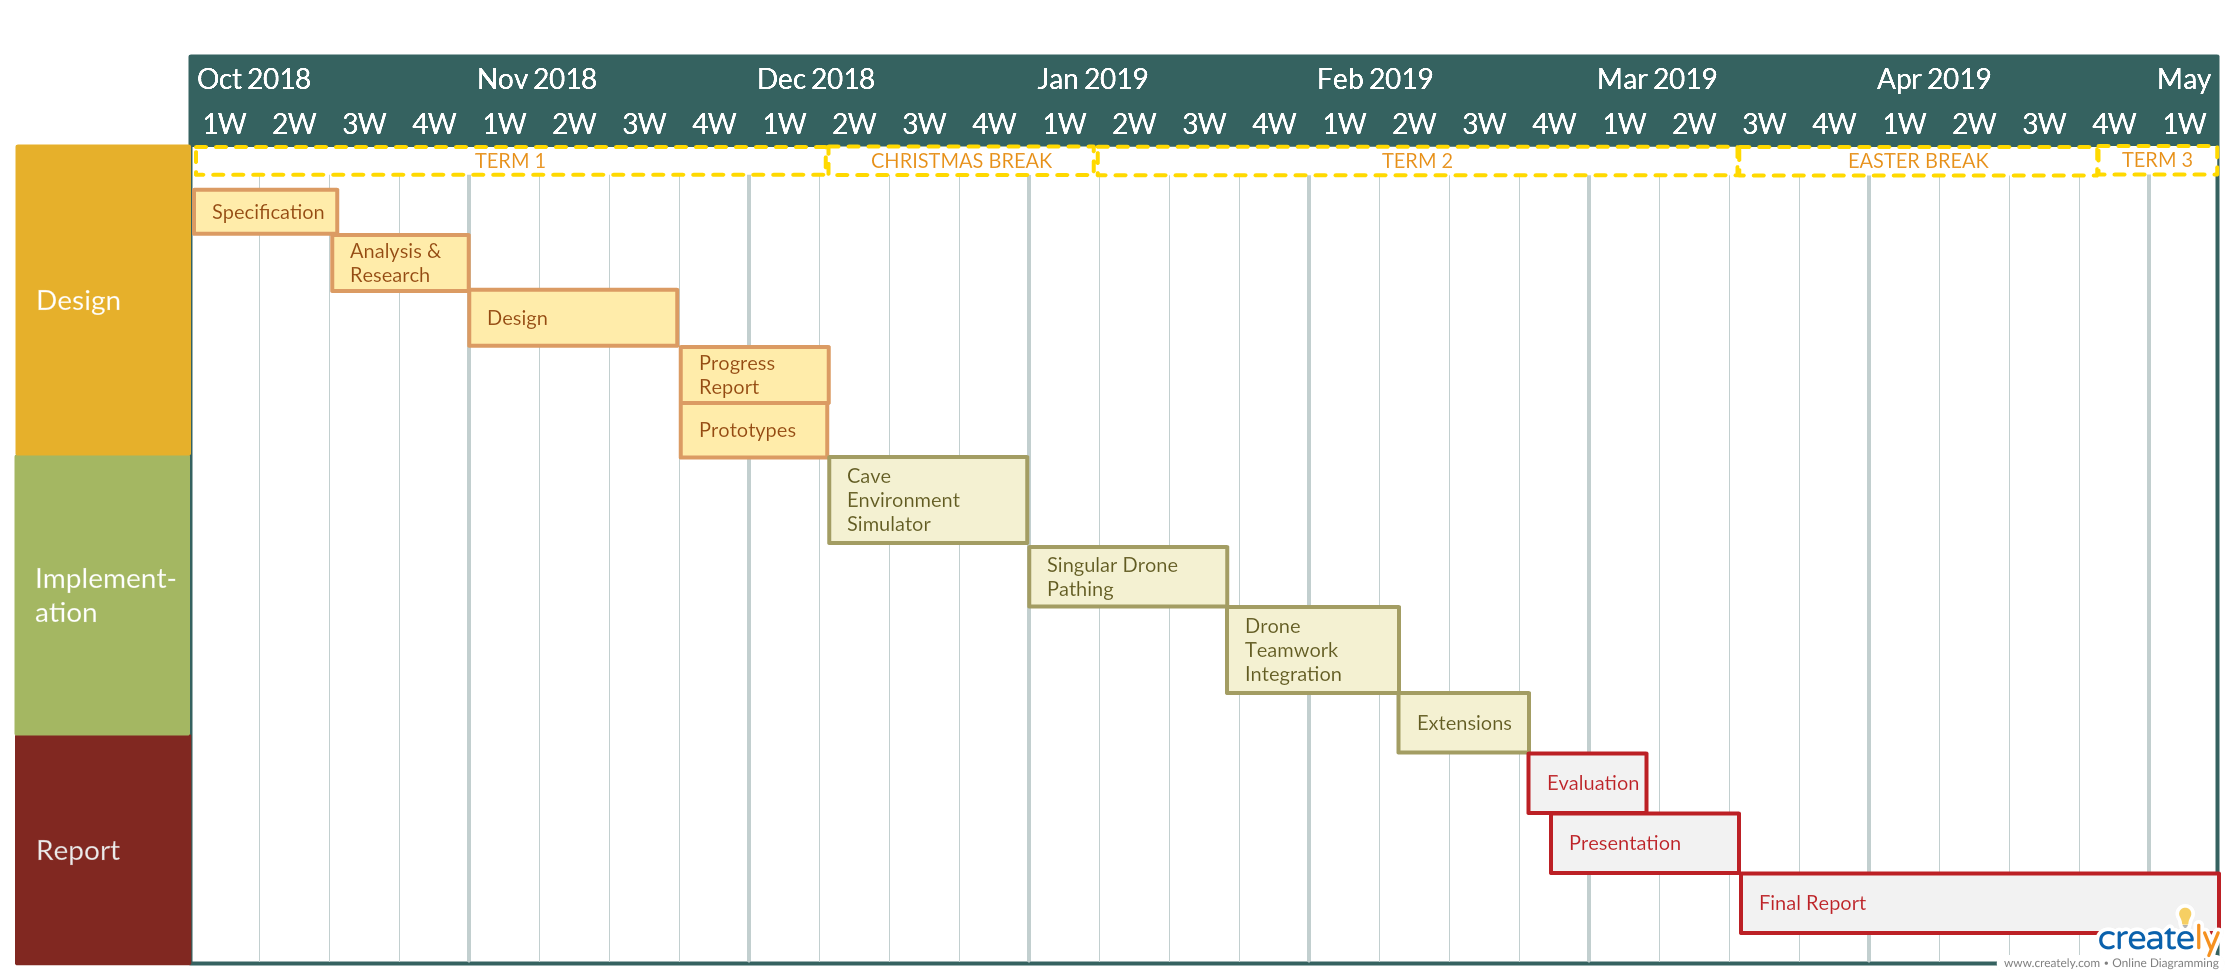
\includegraphics[scale=0.22]{timetable.png}

\section{Risk Assessment}
Illness is a highly potential risk that could occur at any stage of production and can severely slow down progress. Currently the schedule offers more dedicated hours to the project than the recommended amount to account for this risk. Additionally the project is solely dependant on software libraries, and the chosen graphics engine. The risks include the lack of software updates provided by the creator. Using the libraries and engines at a lower version if required will mitigate this risk.

\section{Resources}

\begin{itemize}
    \item Git - For version control of the software and resources.
    \item Github - For storing the git repository remotely. Provides online version control and backups.
    \item Unity - For visualisation of the cavern environment and simulating the navigating drones.
    \item C\#
\end{itemize}

\section{References}

\end{document}
